\section{CPU-level Energy Measurements}
\label{sec:energymeasure}

High precision instruction level energy models can be derived for pipelined
processors by monitoring the instantaneous current drawn by the processor at
each clock cycle, as explained in \cite{nikolaidis2005instruction}. Modern
processors commonly operate at a few GHz, and the Nyquist-Shannon sampling theorem
\cite{nyquist1928certain} states that the sampling frequency must be at least
twice the frequency of the signal being measured. The signal sampled from the
processor might change at least once per clock cycle, so obtaining accurate
measurements would require use of very expensive instruments.

\begin{figure}[tbh]
    \centering
    \includegraphics[width=0.8\textwidth]{figs/shunt.jpg}
    \caption{The shunt resistor used in our experiments.}
    \label{fig:shunt}
\end{figure}

In \cite{rundehvatum2013exploring}, single instructions were measured by
exploiting fast-loop-mode \cite{a9whitepaper} and looping over a group of equal
instructions. A bench multimeter were used to measure the voltage drop over a
shunt resistor like \autoref{fig:shunt}, setup as in \autoref{fig:setup}. From
this, we infer the current flowing from the $V_{core}$ power rail and through
the processor core. The peripherals are isolated and not part of the
measurements. The shunt resistor is chosen such that the voltage drop over it
resides in the range 0 -- 100~mV. According to the datasheet
\cite{agilent34410a}, the voltage readings will have a margin of error of
0.003~\%.

\begin{figure}[bth]
    \centering
    \input{figs/test_setup.tex}
    \caption{Experiment setup for measuring single instruction current drain.}
    \label{fig:setup}
\end{figure}

The use of a shunt resistor to infer current is equivalent to how ammeters work
internally. However, the internal shunt resistor is not scaled for the dynamic
range of a specific target. Also, a too large resistor would drop the voltage
relative to the impedance in the load, and in the case of a processor this can
give unpredictable results. \autoref{fig:varcurrent} illustrates two scenarios
where voltage drops over a $0.1~\Omega$ shunt resistor and a variable load (e.g.
the CPU core). There is a trade-off between accuracy in measurements and voltage
variations across the circuit. If the shunt resistor is too small, the voltage
drop diminishes and is impossible to measure.

\begin{figure}[tbh]
    \centering
    \input{figs/varcurrent.tex}
    \caption{The red and green lines represents two snapshots in time with
    different variable loads. A higher current drain through the circuit
    changes the ratio of voltage drop between the two loads.}
    \label{fig:varcurrent}
\end{figure}

\autoref{fig:consumption} presents results from \cite{rundehvatum2013exploring},
and shows how different instructions use a different amount of energy. This
indicates that the architecture impacts how efficient each instruction is.
$base$ refers to the cheapest instruction in the ISA and roughly corresponds to
the static power consumption.

\begin{figure}[tbh]
    \begin{subfigure}[b]{0.48\textwidth}
        \includegraphics[width=\textwidth]{graph_01_base_cond-0c6.eps}
        \caption{Conditional execution (eq is false).}
        \label{fig:consumptioncond}
    \end{subfigure}
    \begin{subfigure}[b]{0.52\textwidth}
        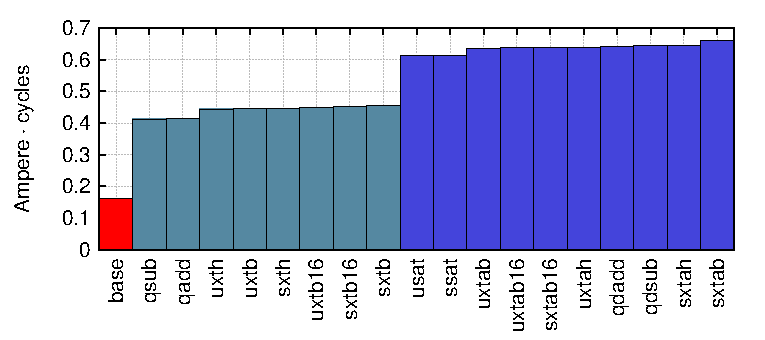
\includegraphics[width=\textwidth]{graph_023_base_quad_saturate_extend-0c6.eps}
        \caption{Non-multiply multi-cycle instructions.}
        \label{fig:consumptionmulti}
    \end{subfigure}
    \caption{Figures from \cite{rundehvatum2013exploring} showing the results of
        measuring the current drain through the CPU core while running isolated
        instructions in a loop. The values are measured current drain multiplied
        by the average number of cycles used.}
    \label{fig:consumption}
\end{figure}


